
		
	\chapter{Pruning unreachable values -uv}
	
	This reduction does delete relaxation to test whether some each fact is reachable and each operation is applicable. If a fact or operation is not reachable nor applicable in the delete relaxation, then it cannot be used in plan without delete relaxation neither with it. Therefore such facts and operations can be removed. 
	
	\begin{figure}
		\begin{subfigure}[b]{0.4\textwidth}
			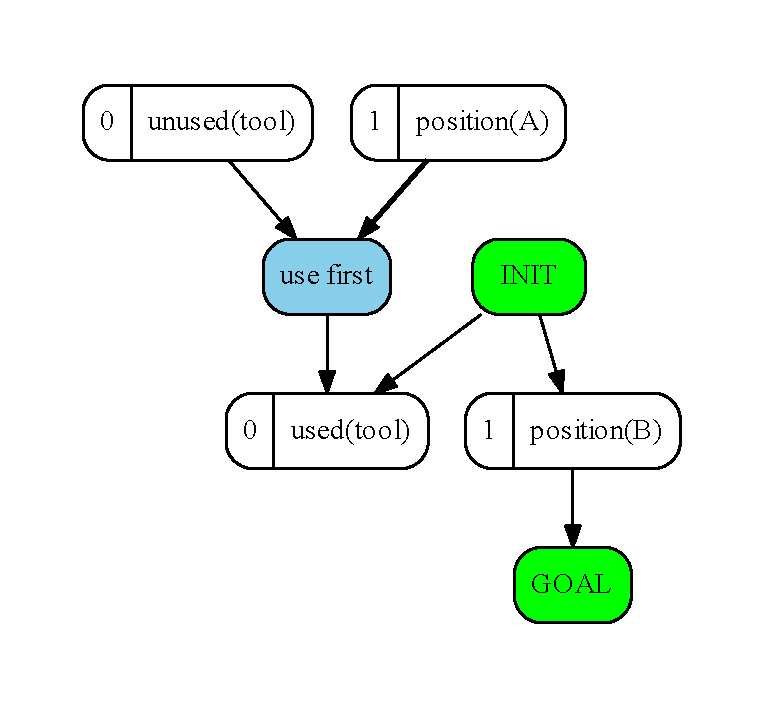
\includegraphics[scale=0.4]{unreachableValues/figures/simple_input}
			\caption{before reduction}
		\end{subfigure}	
		\begin{subfigure}[b]{0.4\textwidth}
			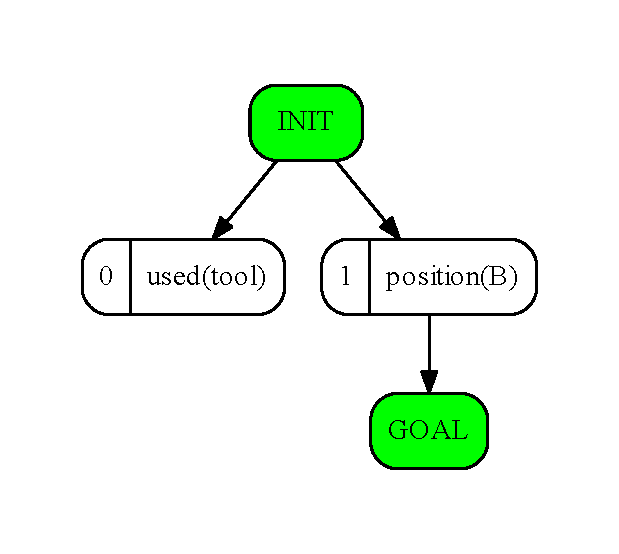
\includegraphics[scale=0.4]{unreachableValues/figures/simple_output}
			\caption{after reduction}
		\end{subfigure}
		\caption{Facts \emph{0 unused(tool)} is unreachable, therefore action \emph{use first} is not applicable. Fact \emph{1 position(A)} is unreachable as well. So these facts and action can be removed. }
	\end{figure}
	
	\section{Reduce operation}
	Let's have SAS in form $<\vars, \init, \goal, \actions, \mutexes{}>$.  Firstly, this operation does delete relaxation by DFS search. The DFS firstly marks all values form $\init$ as reachable and then applies each applicable action and marks its values from $add$ as reachable. Moreover it removes the applied action from the set of action over which it iterates (it is filled by $\actions$ in the beginning). This procedure iterates untill there are no applicable action in the set . After DFS is processed, it has got two sets; set of unreachable values $\vals{}_u$ and set of unreachable actions $\actions{}_u$. Note, that in $\vals{}_u$ there is no value from $\init$. Now, the reduction does following things:
	
	\begin{enumerate}
		\item for each $u \in \vals{}_u$: $u$ is removed from domains ($\vars{}'$ contains variable after this operatiron)
		\item each $u \in  \vals{}_u$ is removed from mutexes ($\mutexes{}'$ contains mutexes after this operation)
		\item $\actions{}' \leftarrow \actions \setminus \actions{}_u$
	\end{enumerate}
	
	Output of the reduction is SAS $<\vars{}', \init{}, \goal{}, \actions{}', \mutexes{}'>$.
	
	\section{Possible outgoing states of SAS}
	\begin{enumerate}
		\item mutex may be empty after this operation
		\item check for removing value from $\goal$ is not implemented, since we assume only plannable instances
		\item possible states of SAS for application of delete variable -dv or merging operators -mo
	\end{enumerate}
	
	\section{States before application of this operation}
	\begin{itemize}
		\item SAS from the beginning
		\item when an effect is removed from action and the value that is added by the effect is not removed (implementation note)
	\end{itemize}
	
	\section{Reverse operation}
	During reverse operation, $\actions{}_u$ are added back to $\actions$ and $\vals{}_u$ are added back to $\vals$ and $\mutexes$.
	
	\section{Implementation notes}
	While removing operators we assume that all operators were active before calling -uv. 
	
	
	
	